%!TEX program = xelatex
\documentclass[8pt, landscape, a4paper]{extarticle}

% --- 核心宏包 ---
\usepackage[UTF8, fontset=fandol]{ctex}
\usepackage[margin=0.8cm, top=1cm, bottom=1.3cm]{geometry}
\usepackage{multicol}
\usepackage{xcolor}
\usepackage{tcolorbox}
\usepackage{enumitem}
\usepackage{amsmath}
\usepackage{amssymb}
\usepackage{fontspec}
\usepackage{tikz}
\usetikzlibrary{arrows.meta, shapes}

% --- 去掉页码 ---
\pagestyle{empty}

% --- 颜色定义 (Purple 主题) ---
\definecolor{headerblue}{RGB}{142, 68, 173}    % Purple
\definecolor{navcolor}{RGB}{211, 84, 0}        % 导航橙
\definecolor{intuitioncolor}{RGB}{41, 128, 185}% 直觉蓝
\definecolor{accentcolor}{RGB}{192, 57, 43}    % 强调红
\definecolor{section2}{RGB}{22, 160, 133}      % 绿色
\definecolor{dividergray}{RGB}{220, 220, 220}

% --- 全局设置 ---
\setlength{\parindent}{0pt}
\setlength{\columnsep}{0.4cm} 
\linespread{1.1} 

% --- 列表样式 ---
\setlist[itemize]{leftmargin=1.2em, nosep, itemsep=2pt, topsep=2pt, label=$\textcolor{headerblue}{\vcenter{\hbox{\tiny$\bullet$}}}$ }
\setlist[description]{leftmargin=0.2em, style=sameline, nosep, itemsep=2pt, font=\bfseries}

% --- Box 样式 ---
\newtcolorbox{mybox}[2][]{%
  colback=white,
  colframe=#2,
  coltitle=white,
  boxrule=1pt,             
  arc=2mm,                 
  left=4pt, right=4pt, top=3pt, bottom=3pt, 
  toptitle=3pt, bottomtitle=3pt, 
  fonttitle=\bfseries\sffamily\large,
  title={#1},
  after skip=5pt          
}

% --- 自定义命令 ---
\newcommand{\subt}[1]{{\vspace{2pt}\textbf{\large \textcolor{black}{#1}}}}

\newcommand{\boxdesc}[1]{%
    \textit{\small \textcolor{gray}{#1}}%
    \par\vspace{2pt}%
    {\color{dividergray}\hrule height 0.5pt}%
    \vspace{2pt}%
}

\newcommand{\sepline}{%
    \par \vspace{3pt}%
    {\color{dividergray}\hrule height 0.5pt}%
    \par \vspace{3pt}%
}

% 公式间距
\setlength{\abovedisplayskip}{3pt}
\setlength{\belowdisplayskip}{3pt}

\begin{document}

% --- 页眉 ---
\begin{center}
    {\Huge \textbf{\sffamily \textcolor{headerblue}{拉普拉斯与Z变换 Laplace \& Z Transforms Cheat Sheet}}} \\
    \vspace{0.2cm}
    {\large \texttt{System Analysis: Stability, Control, and Feedback}}
\end{center}

% --- 开始四栏布局 ---
\begin{multicols*}{4}

% === 第一栏 ===

\begin{mybox}[️ 场景导航 (Use Cases)]{navcolor}
    \boxdesc{遇到什么问题 $\to$ 用什么工具}
    \begin{itemize}[itemsep=2pt]
        \item \textbf{解微分方程 (ODE)} $\to$ 拉普拉斯变换
        \item \textbf{解差分方程 (递推)} $\to$ Z 变换
        \item \textbf{控制系统设计 (PID)} $\to$ 传递函数 $H(s)$
        \item \textbf{数字滤波器 (DSP)} $\to$ 传递函数 $H(z)$
        \item \textbf{系统稳定性分析} $\to$ 极点位置 (Poles)
    \end{itemize}
\end{mybox}

\begin{mybox}[1. 拉普拉斯变换 (Laplace)]{headerblue}
    \boxdesc{连续系统的代数化}
    
    \subt{定义 (单边)}
    $$ F(s) = \int_{0}^{\infty} f(t) e^{-st} dt, \quad s = \sigma + i\omega $$
    \begin{itemize}
        \item \textbf{收敛域 (ROC)}: 使得积分收敛的 $s$ 区域 ($\text{Re}(s) > \sigma_0$)。
        \item \textbf{本质}: 傅里叶变换 + 指数衰减因子 $e^{-\sigma t}$ (处理发散信号)。
    \end{itemize}
    \sepline
    
    \subt{核心性质}
    \begin{itemize}
        \item \textbf{微分}: $f'(t) \iff sF(s) - f(0)$。
        \item \textbf{积分}: $\int f(t) dt \iff \frac{1}{s}F(s)$。
        \item \textbf{终值定理}: $\lim_{t\to\infty} f(t) = \lim_{s\to 0} sF(s)$。
    \end{itemize}
\end{mybox}

\begin{mybox}[2. Z 变换 (Z-Transform)]{headerblue}
    \boxdesc{离散系统的代数化}
    
    \subt{定义 (单边)}
    $$ X(z) = \sum_{n=0}^{\infty} x[n] z^{-n}, \quad z = re^{i\omega} $$
    \begin{itemize}
        \item \textbf{关系}: $z = e^{sT}$ (从 s 平面映射到 z 平面)。
        \item \textbf{单位圆}: 对应 s 平面的虚轴。
    \end{itemize}
    \sepline
    
    \subt{核心性质}
    \begin{itemize}
        \item \textbf{移位}: $x[n-k] \iff z^{-k}X(z)$ (延迟 $k$ 拍)。
        \item \textbf{卷积}: $x[n] * h[n] \iff X(z)H(z)$。
    \end{itemize}
\end{mybox}

\columnbreak

% === 第二栏 ===

\begin{mybox}[3. 传递函数与稳定性 (Stability)]{headerblue}
    \boxdesc{极点决定命运}
    
    \subt{传递函数 (Transfer Function)}
    $$ H(s) = \frac{Y(s)}{X(s)} = \frac{N(s)}{D(s)} = K \frac{\prod (s-z_i)}{\prod (s-p_i)} $$
    \begin{itemize}
        \item \textbf{零点 (Zeros, $z_i$)}: 让输出为 0 的点 (分子根)。
        \item \textbf{极点 (Poles, $p_i$)}: 让输出无穷大的点 (分母根)。
    \end{itemize}
    \sepline
    
    \subt{稳定性判据}
    系统冲激响应 $h(t)$ 是否收敛?
    \begin{itemize}
        \item \textbf{S 域 (连续)}: 所有极点实部 $< 0$ (左半平面)。
        \item \textbf{Z 域 (离散)}: 所有极点模 $< 1$ (单位圆内)。
    \end{itemize}
    \textit{直觉: 极点是系统的“本征模态”,实部正意味着指数增长爆炸。}
\end{mybox}

\begin{mybox}[4. 控制理论基础 (Control)]{headerblue}
    \boxdesc{让系统听话}
    
    \subt{反馈控制 (Feedback)}
    闭环传递函数:
    $$ T(s) = \frac{G(s)}{1 + G(s)H(s)} $$
    \textit{目标: 通过设计控制器 $H(s)$ 移动闭环极点到左半平面。}
    \sepline
    
    \subt{频率响应 (Bode Plot)}
    令 $s = i\omega$。
    \begin{itemize}
        \item \textbf{幅频}: $20 \log |H(i\omega)|$ (dB)。
        \item \textbf{相频}: $\angle H(i\omega)$。
        \item \textbf{带宽}: 增益下降 3dB 的频率。
    \end{itemize}
    \sepline
    
    \subt{PID 控制器}
    $$ C(s) = K_p + \frac{K_i}{s} + K_d s $$
    \begin{itemize}
        \item $K_p$: 比例 (现在的偏差)
        \item $K_i$: 积分 (历史的累积)
        \item $K_d$: 微分 (未来的趋势)
    \end{itemize}
    \sepline
    
    \subt{奈奎斯特判据 (Nyquist)}
    通过开环传递函数的频率响应判断闭环稳定性。
\end{mybox}

\columnbreak

% === 第三栏 ===

\begin{mybox}[5. 常用变换对 (Pairs)]{headerblue}
    \boxdesc{查表神器}
    
    \begin{tabular}{l|l|l}
    \textbf{信号} & \textbf{Laplace ($F(s)$)} & \textbf{Z ($X(z)$)} \\ \hline
    $\delta(t), \delta[n]$ & $1$ & $1$ \\
    $u(t), u[n]$ & $1/s$ & $\frac{z}{z-1}$ \\
    $e^{-at}, a^n$ & $\frac{1}{s+a}$ & $\frac{z}{z-a}$ \\
    $\sin(\omega t)$ & $\frac{\omega}{s^2+\omega^2}$ & $\frac{z \sin \omega}{z^2 - 2z\cos\omega + 1}$ \\
    $t, n$ & $1/s^2$ & $\frac{z}{(z-1)^2}$ \\
    \end{tabular}
    \vspace{3pt}
    \textit{注: Z变换中通常 $a$ 对应 $e^{-aT}$。}
\end{mybox}

\begin{mybox}[6. 滤波器设计 (Filters)]{headerblue}
    \boxdesc{雕刻频率}
    
    \subt{模拟滤波器}
    \begin{itemize}
        \item \textbf{低通}: $H(s) = \frac{\omega_c}{s+\omega_c}$ (一阶)。
        \item \textbf{巴特沃斯}: 通带最平坦。
    \end{itemize}
    \sepline
    
    \subt{数字滤波器}
    \begin{itemize}
        \item \textbf{IIR (无限冲激)}: 有反馈,有极点,可能不稳定。
        \item \textbf{FIR (有限冲激)}: 无反馈,全零点,永远稳定,线性相位。
        \item \textbf{双线性变换}: $s = \frac{2}{T} \frac{1-z^{-1}}{1+z^{-1}}$ (模拟转数字)。
    \end{itemize}
    \sepline
    
    \subt{窗函数设计法}
    FIR 滤波器设计: 理想频率响应 $\to$ IFFT $\to$ 加窗。
    \textit{常用窗: Hamming, Hanning, Blackman。}
    \sepline
    
    \subt{切比雪夫滤波器}
    等波纹特性: 通带或阻带有均匀的纹波。
    \textit{优势: 过渡带更陡峭,阶数更低。}
\end{mybox}

\begin{mybox}[7. Python / Scipy 实战]{headerblue}
    \boxdesc{代码工具箱}
    \begin{itemize}
        \item \texttt{sys = scipy.signal.lti([num], [den])}
        \item \textbf{阶跃响应}: \texttt{step(sys)}
        \item \textbf{波特图}: \texttt{bode(sys)}
        \item \textbf{极零点}: \texttt{sys.zeros, sys.poles}
        \item \textbf{Z变换}: \texttt{scipy.signal.dlsim}
    \end{itemize}
\end{mybox}

\columnbreak

% === 第四栏 ===

\begin{mybox}[8. 高阶视角 (Advanced)]{headerblue}
    \boxdesc{深入系统本质}
    
    \subt{状态空间 (State Space)}
    现代控制理论的核心。
    $$ \dot{x} = Ax + Bu, \quad y = Cx + Du $$
    \begin{itemize}
        \item $A$: 系统矩阵 (特征值即极点)。
        \item \textbf{可控性}: 能否把状态推到任意值?
        \item \textbf{可观性}: 能否通过输出推断状态?
    \end{itemize}
    \sepline
    
    \subt{根轨迹 (Root Locus)}
    随增益 $K$ 变化,闭环极点在复平面上的移动轨迹。
\end{mybox}

\vspace*{\fill}

\begin{mybox}[ 核心直觉 (Intuition)]{intuitioncolor}
    \boxdesc{“S平面是系统的地形图。”}
    
    % TikZ 矢量图: S平面与Z平面的映射
    \begin{center}
    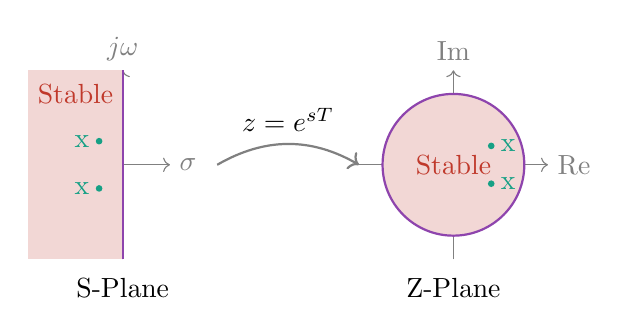
\begin{tikzpicture}[scale=0.6]
        % S Plane
        \begin{scope}[xshift=-3.5cm]
            \draw[->, gray] (-2,0) -- (1,0) node[right] {$\sigma$};
            \draw[->, gray] (0,-2) -- (0,2) node[above] {$j\omega$};
            \fill[accentcolor!20] (-2,-2) rectangle (0,2);
            \node[accentcolor] at (-1,1.5) {Stable};
            \draw[thick, headerblue] (0,-2) -- (0,2);
            \node[below] at (0,-2.2) {S-Plane};
            \fill[section2] (-0.5, 0.5) circle (2pt) node[left] {x};
            \fill[section2] (-0.5, -0.5) circle (2pt) node[left] {x};
        \end{scope}
        
        % Mapping Arrow
        \draw[->, thick, gray] (-1.5, 0) to[bend left] (1.5, 0);
        \node[above] at (0, 0.5) {$z = e^{sT}$};
        
        % Z Plane
        \begin{scope}[xshift=3.5cm]
            \draw[->, gray] (-2,0) -- (2,0) node[right] {Re};
            \draw[->, gray] (0,-2) -- (0,2) node[above] {Im};
            \draw[thick, headerblue, fill=accentcolor!20] (0,0) circle (1.5cm);
            \node[accentcolor] at (0,0) {Stable};
            \node[below] at (0,-2.2) {Z-Plane};
            \fill[section2] (0.8, 0.4) circle (2pt) node[right] {x};
            \fill[section2] (0.8, -0.4) circle (2pt) node[right] {x};
        \end{scope}
    \end{tikzpicture}
    \end{center}

    \hspace{1em}拉普拉斯变换将随时间变化的\textbf{微分方程}变成了静态的\textbf{代数方程}。
    \vspace{4pt}
    
    \subt{三大核心视角}
    \begin{itemize}[itemsep=4pt]
        \item \textbf{极点即寿命}: 
        极点的实部决定了信号是衰减 (稳定) 还是增长 (爆炸)。极点离虚轴越远,衰减/增长越快。
        
        \item \textbf{虚部即频率}: 
        极点的虚部决定了震荡的频率。共轭极点对产生正弦震荡。
        
        \item \textbf{映射即离散化}: 
        Z 变换就是把 S 平面的左半平面“卷”成了一个单位圆。虚轴变成了圆周。这就是为什么离散系统的稳定性看单位圆。
    \end{itemize}
    
    \vspace{6pt}
    \centering\textit{\footnotesize 给我极点的位置,我就能预言系统的未来。}
\end{mybox}

\end{multicols*}

\end{document}
